\centering
\usetikzlibrary{calc}

\definecolor{cb3b3b3}{RGB}{179,179,179}
\definecolor{ccccccc}{RGB}{204,204,204}
\definecolor{cffffff}{RGB}{255,255,255}

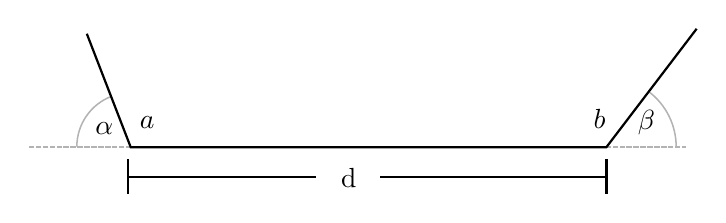
\begin{tikzpicture}[y=0.80pt,x=0.80pt,yscale=-1, inner sep=0pt, outer sep=0pt]
\centering

  \path[draw=cb3b3b3,dash pattern=on 2pt off 0.5pt,line join=miter,line
    cap=butt,miter limit=4.00,dash phase=0.201pt,line width=0.800pt]
    (115.9129,172.6241) -- (69.8665,172.6241);
  \path[draw=cb3b3b3,dash pattern=on 2pt off 0.5pt,line join=miter,line
    cap=butt,miter limit=4.00,dash phase=0.201pt,line width=0.800pt]
    (330.6888,172.6195) -- (366.5496,172.6195);
  \path[cm={{1.45393,0.0,0.0,1.45393,(-471.01666,-377.22731)}},draw=cb3b3b3,miter
    limit=4.00,line width=0.550pt] (564.5997,360.8878)arc(-52.961:0.593:21.466);
  \path[cm={{0.52395,0.0,0.0,0.52395,(41.81533,-25.47312)}},draw=cb3b3b3,miter
    limit=4.00,dash phase=8pt,line width=0.55pt]
    (94.9543,377.5908)arc(179.987:249.624:46.467);
  \path[fill=black,line width=0.800pt] (100,167) node[above right]
    (text4046) {$\alpha$};
  \path[fill=black] (345,167) node[above right] (text4046-2)
    {$\beta$};
  \path[draw=black,line join=miter,line cap=butt,line width=0.800pt]
    (114.8543,177.9195) -- (114.8543,193.7975);
  \path[draw=black,line join=miter,line cap=butt,line width=0.800pt]
    (114.8543,186.1205) -- (330.7957,186.1205);
  \path[draw=black,line join=miter,line cap=butt,line width=0.800pt]
    (330.7957,177.9195) -- (330.7957,193.7975);
  \path[fill=cffffff,line width=0.800pt,rounded corners=0.0000cm]
    (199.5575,177.5072) rectangle (228.2820,192.5707);
  \path[fill=black,line width=0.800pt] (211,191) node[above right]
    (text4081) {d};
  \path[draw=black,line join=miter,line cap=butt,line width=0.800pt]
    (96.0814,121.3474) -- (115.9166,172.6195) -- (330.7355,172.6195) --
    (371.5287,119.1019);
      \path[] (120,164) node[above right]
    (text4046) {$a$};
      \path[] (325,164) node[above right]
    (text4047) {$b$};
\end{tikzpicture}
\caption{Variables for the connection between two elements at points $a$ and $b$: tangents $\alpha$ and $\beta$ and distance $d$}
